\nonstopmode		% added to ignore some compiling errors...

% ---------------------------------------------------------------------------
% Author guideline and sample document for EG publication using LaTeX2e input
% D.Fellner, v1.13, Jul 31, 2008

\documentclass{egpubl}
\usepackage{pg2015}


% --- for  Annual CONFERENCE
% \ConferenceSubmission % uncomment for Conference submission
% \ConferencePaper      % uncomment for (final) Conference Paper
% \STAR                 % uncomment for STAR contribution
% \Tutorial             % uncomment for Tutorial contribution
% \ShortPresentation    % uncomment for (final) Short Conference Presentation
%
% --- for  CGF Journal
% \JournalSubmission    % uncomment for submission to Computer Graphics Forum
% \JournalPaper         % uncomment for final version of Journal Paper
%
% --- for  CGF Journal: special issue
% \SpecialIssueSubmission    % uncomment for submission to Computer Graphics Forum, special issue
% \SpecialIssuePaper         % uncomment for final version of Journal Paper, special issue
%
% --- for  EG Workshop Proceedings
 \WsSubmission    % uncomment for submission to EG Workshop
% \WsPaper         % uncomment for final version of EG Workshop contribution
%
 \electronicVersion % can be used both for the printed and electronic version

% !! *please* don't change anything above
% !! unless you REALLY know what you are doing
% ------------------------------------------------------------------------

% for including postscript figures
% mind: package option 'draft' will replace PS figure by a filename within a frame
\ifpdf \usepackage[pdftex]{graphicx} \pdfcompresslevel=9
\else \usepackage[dvips]{graphicx} \fi

\PrintedOrElectronic

% prepare for electronic version of your document
\usepackage{t1enc,dfadobe}

\usepackage{egweblnk}
\usepackage{cite}

% For backwards compatibility to old LaTeX type font selection.
% Uncomment if your document adheres to LaTeX2e recommendations.
% \let\rm=\rmfamily    \let\sf=\sffamily    \let\tt=\ttfamily
% \let\it=\itshape     \let\sl=\slshape     \let\sc=\scshape
% \let\bf=\bfseries

% end of prologue

% !TEX root = ./EGauthorGuidelines-pg2015-sub.tex


% ---------------------------------------------------------------------
% EG author guidelines plus sample file for EG publication using LaTeX2e input
% D.Fellner, v1.17, Sep 23, 2010


\usepackage[]{lineno}
\usepackage{lipsum}
\usepackage{amsmath}
\usepackage{amsmath,amsfonts}
\usepackage{amssymb}
\usepackage{rotating}


% MyDefs

\newcommand\ie{{\em i.e.}}
\newcommand\eg{{\em e.g.}}

\newcommand\red{\color{red}}
\newcommand\green{\color{OliveGreen}}
\newcommand\blue{\color{blue}}
\newcommand\brown{\color{Brown}}
\newcommand\orange{\color{RedOrange}}
\newcommand\wrong[1]{{\color{red}#1}}


\newcommand\remove[1]{{\red \sout{#1}}}
\newcommand\removeWnote[2]{{\red \sout{#1}} {\textit{\green(#2)}}}
\newcommand\replace[2]{{\red \sout{#1}} {\orange #2}}
\newcommand\add[1]{{\orange #1}}
\newcommand\addWComment[2]{{\orange #1} {\textit{\green(#2)}}}
\newcommand\review[1]{{\blue #1}}
\newcommand\reviewWComment[2]{{\blue #1} {\textit{\green(#2)}}}
\newcommand\addComment[1]{\textit{\green(#1)}}

% ---------------------------------------------------------------------




\title[Visual Simulation of Low-Order Aberrations on Monochromatic Images]{Visual Simulation of Low-Order Aberrations on Monochromatic Images}

% for anonymous conference submission please enter your SUBMISSION ID
% instead of the author's name (and leave the affiliation blank) !!
%\author[paperID]{paperID}

% for anonymous conference submission please enter your SUBMISSION ID
% instead of the author's name (and leave the affiliation blank) !!
\author[M.L. Krueger, M.M. Oliveira \& A.L. Kronbauer]
       {Matheus Luan Krueger, Manuel M. Oliveira and Airton Leite Kronbauer
%        S. Spencer$^2$\thanks{Chairman Siggraph Publications Board}
        \\
% For Computer Graphics Forum: Please use the abbreviation of your first name.
         Institute of Informatics, UFRGS, Brazil\\
         %$^2$Rio Grande do Sul Eye Care Centre, CORS, Brazil
%        $^2$ Another Department to illustrate the use in papers from authors
%             with different affiliations
       }

% ------------------------------------------------------------------------

% if the Editors-in-Chief have given you the data, you may uncomment
% the following five lines and insert it here
%
% \volume{27}   % the volume in which the issue will be published;
% \issue{1}     % the issue number of the publication
% \pStartPage{1}      % set starting page


%-------------------------------------------------------------------------
\begin{document}

%\teaser{
%	
\includegraphics[width=\linewidth]{eg_new}
%	\centering
%	\caption{New EG Logo}
%	\label{fig:teaser}
%}

\maketitle

\begin{abstract}
\textbf{Purpose:} 
To describe a practical approach for modeling and simulating the visual perception of monochromatic images observed by an optical systems with low-aberrations (\ie, myopia, hyperopia and astigmatism)
%a technique capable of simulating the perception of monochromatic images when considering optical systems with low-order aberrations (\ie, myopia, hyperopia and astigmatism). 
%
\textbf{Methods:} 
%
We have created images of Sloan letters at LogMAR (Logarithm of the Minimum Angle of Resolution) values ranging from -0.3 to 1.0 in steps of 0.1. And captured them by using a DSLR camera in order to represent a perfect eye (\ie, without refractive aberrations). We place additional lenses in front of the camera's optical system to induce low-order aberrations. Finally, we characterize the optical aberrations of the human eye using a wavefront aberration function, which is used, together with the images captured by the camera, to perform simulations in the frequency domain. 
%
\textbf{Results:} 
%
To objectively evaluate the quality of the simulated results, we use three objective metrics: the SSIM (Structural Similarity Image Metric), the PSNR (Peak Signal-to-Noise Ratio), and the AD (Absolute Difference) of the pixelwise differences between the captured and simulated images. Considering all simulations, we have obtained a SSIM mean value of 0.93 (minimum of 0.91) and a PSNR mean value of 35.50dB (minimum of 29.50dB).
%
\textbf{Conclusions:} 
%indicates that our simulations indeed produces results that are structurally very similar the ground truth
% indicates that our simulations produce results indistinguishable from the optical ground truth.
The results of the SSIM and PSNR metric confirm that the results produced by our simulations are structurally and perceptually similar to the ground truths captured by the camera.


\begin{keywords}
Low-order aberrations, Fourier Optics, PSF.
\end{keywords}

\end{abstract}



\linenumbers

%-------------------------------------------------------------------------
\section{Introduction}

Vision is the primary channel we use to perceive the universe. Its unique capability allows us to acquire information about the surrounding world by sensing the intensity and color of light. This experience is unique and the perceived image is affected by several individual factors (\eg, refractive errors, light sensitivity, distribution of photoreceptors in the retina, etc.). Simulating visual experience is a complex and difficult task, which requires the integration of a wide range of fields, including optics, anatomy, physiology, biochemistry, psychology, and cognitive neurosciences \cite{Schwartz2010}.

Visual aberrations can be classified as low-order or high-order. Low-order aberrations (\ie, myopia, hyperopia, astigmatism, and presbyopia) can be described in terms of sphero-cylindrical values and can be corrected with the use of eye glasses, contact lenses, or refractive surgery. They are responsible for about 90\% of ones loss of visual acuity \cite{Dias2014}. The remaining 10\% is due to a combination of particular imperfections, known as high-order aberrations (\eg, trefoil, coma, quadrafoil, secondary astigmatism). Visual aberrations can be described by the eye's point-spread function (PSF), often represented using the so-called wavefront maps. Fig.~\ref{fig:eyes} illustrates the human eye and the effects of some low-order aberrations when focusing at infinity.

\begin{figure}[!ht]
	\centering
	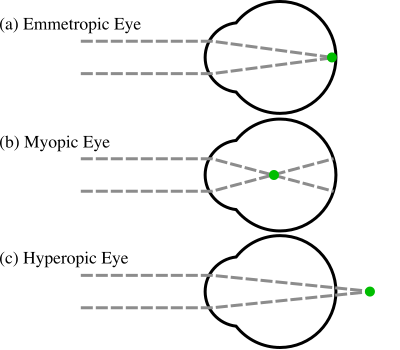
\includegraphics[width=1.00\linewidth]{eyes.png}
	\caption{The human eye and some low-order aberrations. (a) A perfect eye focuses the parallel rays to a single point on the retina; (b) a myopic eye has an elongated eye ball or a bumped cornea, focusing parallel rays at a point before the retina; and (c) a hyperopic eye has a shallow eye ball or a flatter cornea, thus focusing parallel rays at point behind the retina.}
	\label{fig:eyes}
\end{figure}

The simulation of how an impaired eye perceives a scene is a complex, but highly important task. It could, for instance, give doctors an idea of how a given patient's vision was before and after some surgical procedure. It could also allow primary school teachers understand the complaints of their students. In practice, poor visual performance is often misinterpreted as the perception of blurry images. However, the problem is not that simple. Visual simulation is an intricate process that requires sophisticated tools of Fourier analysis \cite{Thibos2011}. From a simple geometrical perspective, when the optical system of an eye is mis-focused at a point in the scene, the light emitted/reflected by such a point is spread out across some area (circle of confusion) of the retinal surface, causing blur. This can be understood from Fig.~\ref{fig:eyes}(b) and \ref{fig:eyes}(c). Note that when the optical system is well focused (Fig.~\ref{fig:eyes}(a)) a point on the scene is imaged to a point on the retina.

Unlike traditional 2-D digital image processing in which an image is blurred by convolving it with a spatially-invariant low-pass filter kernel, visual blurring is a depth-dependent phenomenon (\ie, the amount of blurring introduced by the eye's PSF varies with the distance from the observer's focal plane to the scene element). If depth is not taken into account by the blurring method, the resulting image might be very different from the one formed onto the retina.

\begin{figure*}[hbt]
  \centering
  \mbox{} \hfill
  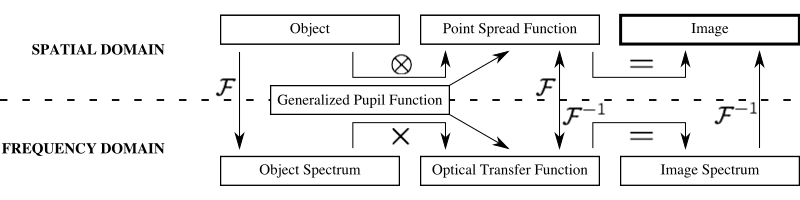
\includegraphics[width=.99\linewidth]{pipeline.png}
  \hfill \mbox{}
  \caption{The pipeline for simulating visual aberrations. It illustrates two paths for computing the retinal image of an object when the point spread function of the eye (PSF), or equivalently, the optical transfer function (OTF), is known. The computation indicated at the top is carried out entirely in the spatial domain. The convolution of image with the PSF gives the retinal image directly. The more efficient computation in the spatial frequency domain is illustrated at the bottom. In that case, the product of the object spectrum (obtained by the Fourier transform of the object) and the optical transfer function is the image spectrum, from which the image itself can be obtained by inverse Fourier transformation. $\mathcal{F}$ and $\mathcal{F}^{-1}$ stands for the Fourier transform and inverse Fourier transform operators.}
	\label{fig:pipeline}
\end{figure*}

We present a practical approach to the problem of simulating how visual low-order aberrations (\ie, myopia, hyperopia and astigmatism) affect the perception of monochromatic images. It relies on the assumption of a fixed depth and uses Fourier Tools and a DSLR camera to simulate and validate results. We demonstrate its effectiveness by comparing the simulation outcomes with an optical ground truth by using three objective metrics.

The main \textbf{contributions} of this paper include:

\begin{itemize}
	\item A description of a technique for modeling and simulating visual aberrations;
	\item A DLSR camera-based approach to validate the visual simulation results.
\end{itemize}


%-------------------------------------------------------------------------
\section{Related Work}

Vision simulation has been addressed in different ways over the years. Since the first synthetic image with depth of field computed by Potmesil and Chakravarty \cite{Potmesil1981}, there has been a significant number of computer graphics techniques addressing the rendering of realistic effects. More recently, the possibility of estimating and compensating for refractive errors has attracted the attention of several researchers, mainly addressing the formulation of interactive, portable, and inexpensive solutions. The following subsections describe the main techniques for simulating, estimating, and correcting visual aberrations.

\subsection{Optical Simulation Techniques}

Barsky \cite{Barsky2004} proposed a method for generating synthetic images incorporating the optical characteristics of an individual. Specifically, his method simulates the perception of an individual based on data acquired using a Shack-Hartmann wavefront aberrometer. Once the wavefront data is captured, it is sampled to calculate an {\it Object Space PSF} (OSPSF) and used to blur the input synthetic scene at different depths.

Many researchers have used raytracing techniques and anatomical optics to study and simulate vision by using theoretical models of the human eye \cite{Camp1990, Kolb1995}. Camp, Maguire and Robb \cite{Camp1990} described two ray tracing algorithms for deriving an optical PSF from corneal topography measurements. They focused on simulating and evaluating optical performance of patients' eyes with the following corneal pathologies: \emph{keratoconus}, \emph{epikeratophakia for aphakia} and \emph{radial keratonomy}. Kolb, Mitchell and Hanrahan \cite{Kolb1995} presented a physically-based camera model that simulates aberration and radiation. To simulate such effects, they compute the geometry of image formation of a particular lens system using a modified distributed ray tracing algorithm. The algorithm is a hybrid of rendering and lens maker techniques, and can produce images of synthetic scenes showing a variety of optical effects. Mostafawy, Kermani and Lubatschowski \cite{Mostafawy1997} combined the algorithm presented by Kolb, Mitchell and Hanrahan \cite{Kolb1995} and the dimensions of an schematic eye model to generate virtual simulations of vision after corrective surgery.

Moreover, the study of monochromatic aberrations of the human eye with wavefront sensors \cite{Liang1994} allowed many others to perform simulations by using Fourier tools to mimic visual perception. Yu \cite{Yu2001} presents a technique capable of generating simulations of synthetic and  real scenes focusing at a specific depth. Instead of considering only the corneal surface and using raytracing techniques to perform such simulations, the authors rely on data captured by a Shack-Hartmann device. With this information his technique construct a wavefront, which is used to blur a sharp image according to a depth map. However, he do not present a proper way of evaluating the simulations' outcomes, which could be, for example, compared with an optical ground truth. Watson and Ahumada Jr \cite{Watson2008} proposed an image-based model for predicting acuity from optical aberrations. In this model, a `neural image' is computed incorporating optical and neural filtering. Then, this image is presented to four human observers and the LogMAR acuity is evaluated. By doing this, they can relate visual acuity as a function of a particular aberration and compute predictions of how a specific aberration (\eg, defocus) affects visual acuity.

\subsection{Non-Optical Simulation Techniques}

Some techniques are concerned with modeling the effects caused by non-optical issues and use them to achieve more realistic synthetic images. One example is the method proposed by Deering \cite{Deering2005}. His approach describes a retinal photon-accurate model of the human eye. Such a model is used together with computer graphics techniques and a simplified eye's optical model to produce synthetic simulations of the image formation process. 

Another technique that explores different effects caused by the anatomy of the human eye --- the glare --- is discussed by Ritschel et al. \cite{Ritschel2009}. The authors proposed a model for a real-time dynamic simulation of the scattering in the human eye, which is efficiently implemented by drawing a few basic primitives, applying an FFT, and doing a special kind of blur. They have also performed psychophysical studies to measure the perception of brightness for glare models. However, they state that, as any other intrinsic phenomena, no ground truth can be obtained. And the model's validation remains a challenging task.

\section{Estimating/Correcting Visual Optical Aberrations}
\label{sec:EstimatingCorrectingVisualOpticalAberrations}

Pamplona et al. \cite{Pamplona2010} presented a practical approach for estimating low-order aberrations without the need of expensive equipments. It uses a pinhole mask attached to a smartphone displaying patterns to the subject. The aberrations are estimated by the subjective alignment of the different patterns.
Kronbauer et al. \cite{Kronbauer2011} developed a psychophysical approach for vision measurement in candelas. It consists in presenting light stimulus in a display in order to discover the absolute threshold for clear and dark conditions. Then, by relating it with an objective vision's assessment (\eg, vision chart acuity and aberrometry data), they have stated a strong correlation between aberrometry data and the absolute threshold.

Many methods have achieved the goal of free the viewer from needing wearable optical correction when looking at displays \cite{Huang2012, Pamplona2012b, Huang2014}, and printings or projections \cite{Montalto2015}. Other works have explored physiologically-based models to provide insights and feedback on how to produce high-fidelity effects and improve visualization experiences \cite{Machado2009, Pamplona2009, Pamplona2011}.


%-------------------------------------------------------------------------
\section{Methods}

This section describes the approach used for visual simulation of low-order refractive errors, and the experimental design. Fig.~\ref{fig:pipeline} illustrates its pipeline, showing equivalent operations specified both in the spatial and in the frequency domain. Since we are primarily interested in visual acuity, all experiments and discussions presented here are based on monochromatic images. As visual blurring is a depth-dependent phenomenon, we have adopted the simplifying assumption that the observed images are at some constant depth. For this, we used two sets of charts containing standard Sloan letters: black letters on white background, as well as white letters on black background.

%-------------------------------------------------------------------------
\subsection{Target Images and Capture Setup}

We have created images of Sloan letters at LogMAR (Logarithm of the Minimum Angle of Resolution) values ranging from -0.3 to 1.0 in steps of 0.1. The LogMAR scale \cite{Bailey1976} provides a more accurate estimate of visual acuity when compared to other charts (\eg, Snellen), being the recommended one for research settings. 
Our target images were created according to Eq.~\ref{eq:lettersize} for testing vision from three feet away. The individual letters were rendered using the vector graphics capabilities of Inkscape and the Sloan PostScript fonts provided by Pelli, Robson et al.\cite{Pelli1988}.
% as well as white letters on black background. 
At the prescribed distance, the ratio between one pixel and one arc minute is 1:1, that is, the letters with a LogMAR value of 0 (or the known Snellen fraction 20/20) has exactly 5 pixels of height. For the purpose of our simulations, each black (white) optotype was placed against a $113 \times 133$-pixel black (white) square.   
Since $1~degree = 60~arc~minutes$, each such square covers a total field of view (FOV) of $1.88^{\circ}~\times~1.88^{\circ}$. The conversion from \emph{Snellen decimal acuity} values  
%and vice-versa are 
to LogMAR values is presented in Eq.~\ref{eq:dec2logmar}. A Snellen decimal acuity value is the decimal representation
of the Snellen fraction (\eg, Snellen ratios of 20/20 and 20/40 correspond to Snellen decimal acuity values of 1.0 and 0.5, respectively). 
% and \ref{eq:logmar2dec}, respectively.

\begin{equation}
	\centering
	\label{eq:lettersize}
	\begin{aligned}
	letter~size_{mm} = 	& ~deg2rad \left (\frac{5}{60} \right ) \\
    	  				& \times (chart~distance_{mm}) \\
      					& \times (10^{-LogMAR})^{-1}
	\end{aligned}
\end{equation}

\begin{equation}
	\centering
	\label{eq:dec2logmar}
	LogMAR = -\log_{10} (Snellen~decimal~acuity)
\end{equation}

We have printed the described white- and black-background LogMAR charts containing Sloan letters specifically designed for a viewing distance of three feet. The charts were printed on white paper using a laser printer at 360 dpi. We then took pictures of the charts with a DSLR camera. The camera was placed at three feet (91.44 cm) from the chart, with focal length set to 18mm. Since images acquired using this setup respect the 1:1 ratio between pixels and arc minutes, one can crop the squares containing the individual optotypes for further processing.

%-------------------------------------------------------------------------
\subsection{Modeling Visual Aberrations}

\begin{figure}[!bh]
	\centering
	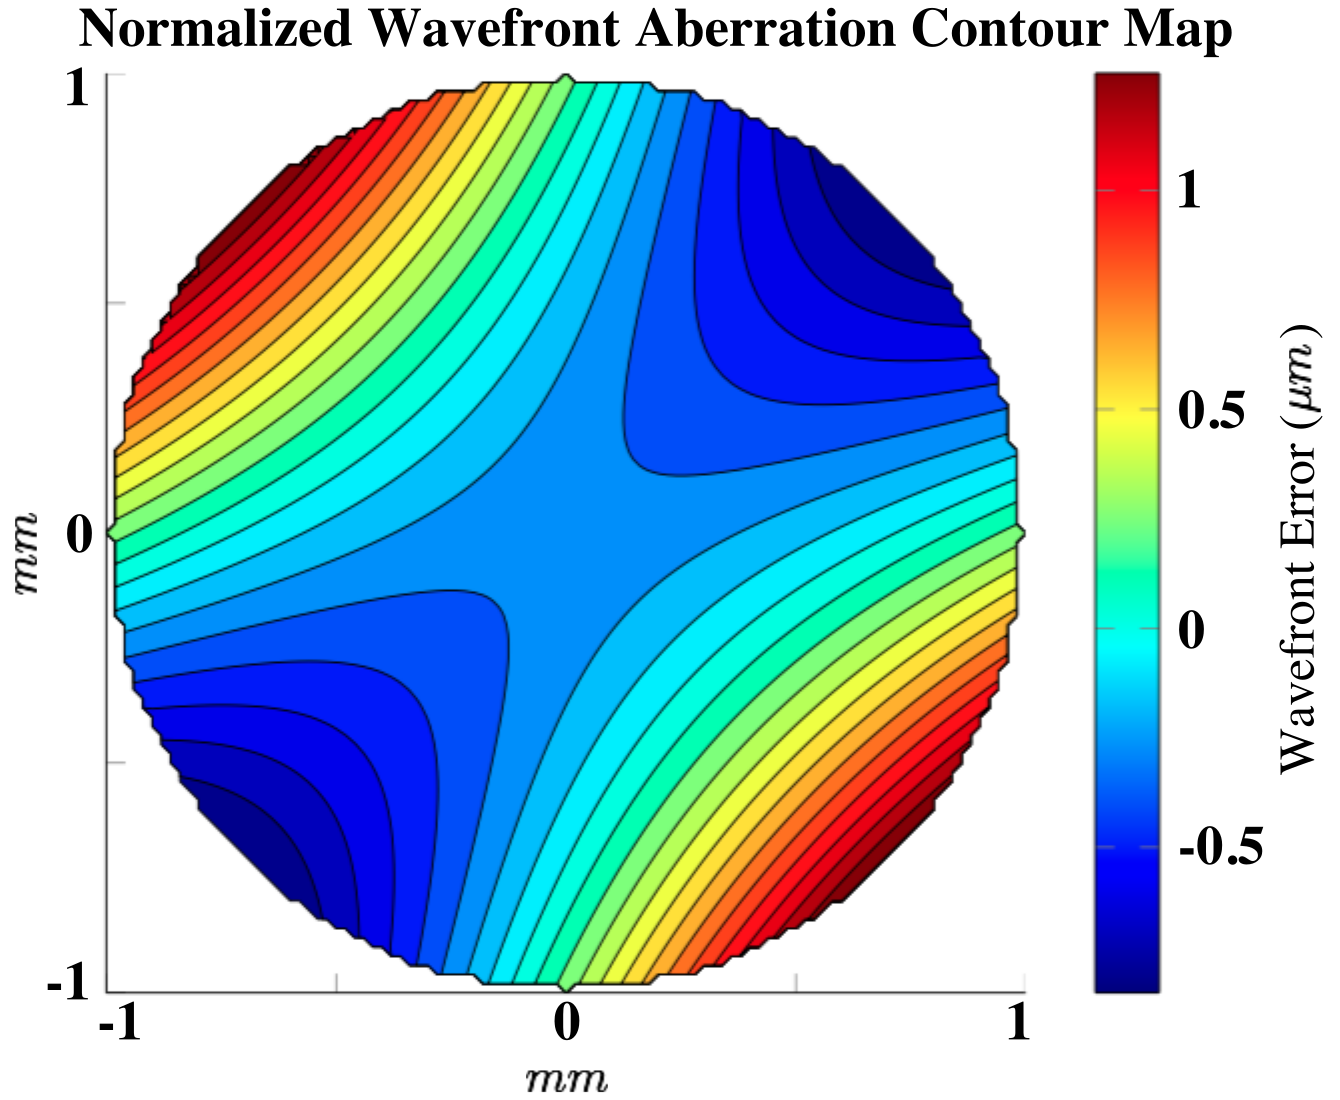
\includegraphics[width=1.00\linewidth]{wavefront.png}
	\caption{Normalized wavefront map for an eye with: S = 0.5D, C = -2.0D, $\phi = 45^\circ$ and R = 1.5mm. The map represents a pupil with a radius of 1.0mm. The root mean square (RMS) wavefront error (in $\mu m$) is the deviation of the wavefront aberration function $W$ (Eq.~\ref{eq:W}) from a plane wave.}
	\label{fig:wavefront}
\end{figure}

We characterize the optical aberrations of the human eye using a wavefront aberration function. Such a function defines a wavefront map, which is approximated using Zernike polynomials. 
Obtaining a complete wavefront function, which models both low-order and high-order aberrations, requires access to expensive wavefront aberrometer devices. In this work, we only consider the low-order aberrations (\ie, myopia, hyperopia, and astigmatism), which can be easily obtained from any eyeglass or contact lens prescription. One should note, however, that low-order aberrations are responsible for about 90\% of one's total visual aberrations~\cite{Dias2014}. This should not come as a surprise, given that eyeglasses only correct for low-order aberrations and are the primary way of achieving corrected 20/20 vision. 
%As a complete wavefront map acquisition requires 
%is quite expensive and not accessible worldwide, 
We obtain wavefront aberration function $W_{(x,y)}$ from prescription data as~\cite{Dai2008}:
%to convert elementary information to wavefront maps: 

\begin{equation}
	\label{eq:W}
	W_{(x,y)} = \sum_{i=-1}^1 c_{2}^{2i} ~ Z_{2}^{2i}_{(x,y)},
\end{equation}
where
\begin{equation}
	\centering
	\label{eq:c2-2}
	c^{-2}_{2} = \frac{R^2*C*\sin(2\phi )}{4\sqrt{6}},
\end{equation}
%
\begin{equation}
	\centering
	\label{eq:c20}
	c^{0}_{2} = - \frac{R^2 * (S + C/2))}{4\sqrt{3}}, 
\end{equation}
%
\begin{equation}
	\centering
	\label{eq:c22}
	c^{2}_{2} = \frac{R^2*C*\cos(2\phi )}{4\sqrt{6}}
\end{equation}

\noindent
and 
$c^{-2}_{2}$, $c^{0}_{2}$, and $c^{2}_{2}$ are the coefficients of the Zernike polynomials corresponding to \emph{oblique astigmatism} ($Z^{-2}_{2}$), \emph{defocus} ($Z^{0}_{2}$), and \emph{vertical astigmatism} ($Z^{2}_{2}$), respectively.
$S$, and $C$ are respectively the \emph{sphere} and \emph{cylinder} values that specify the optical power in diopters (D).  $\phi$ is cylinder axis expressed in degrees. 
%Both $S$ and $C$ are in diopters,
The values $S$, $C$, and $\phi$ are popularly referred to as the "degree", the "astigmatism", and the "axis of astigmatism" in one's prescription. 
$R$ is the radius of the subject's pupil (an aperture, in general)  measured in mm, and $c^{-2}_{2}$, $c^{0}_{2}$ and $c^{2}_{2}$ are in $\mu$m. Fig.~\ref{fig:wavefront} illustrates a wavefront map obtained for $S = 0.5$D, $C = -2.0$D, $\phi = 45^\circ$ and $R = 1.5$mm. If no aberration is present, the resulting wavefront is planar.
% (zero error).


%-------------------------------------------------------------------------

\subsection{Image Filtering}

Given $S$, $C$, $R$, and $\phi$,  
one can obtain the effective aberration function as $kW_{(x,y)}$, where $k$ is the spherical wavenumber (\ie, $k = 2\pi/\lambda$), and 
$W_{(x,y)}$ is the wavefront aberration function expressed using the Zernike polynomials. For the case of low-order aberrations, $W_{(x,y)}$ is defined by \review{Eq.~\ref{eq:W}}, which takes into account oblique astigmatism, defocus, and vertical astigmatism. 
 $\lambda = 550nm$ is a standard wavelength used for monochromatic simulation \cite{Dai2008}.
 The pupil function $P_{(x,y)}$ is a binary  function that evaluates to 1 inside the projected aperture, and 0 outside it. According to Goodman \cite{Goodman2005}, the \emph{generalized pupil function} $\mathbb{P}_{(x,y)}$ is given by:
 
\begin{equation}
	\centering
	\label{eq:generalizedpupilf}
	\mathbb{P}_{(x,y)} = P_{(x,y)} \exp[j*k*W_{(x,y)}],
\end{equation}
%
where $j = \sqrt{-1}$. Note that $\mathbb{P}_{(x,y)}$ is a complex number. One can obtain the point spread function of the optical system as the power spectrum of $\mathbb{P}$, \ie,  $PSF = \left | \mathcal{F}(\mathbb{P}) \right | ^ {2}$, where $\mathcal{F}$ is the Fourier transform operator.  Given the PSF and 
an input image $I$, one can simulate the view of $I$ through the given optical system computing the 2-D convolution
$O = PSF \otimes I$.
A more efficient computation of $O$ can be obtained in the frequency domain (this is illustrated by bottom path in Fig.~\ref{fig:pipeline}). In that case, $O = \mathcal{F}^{-1}(\mathcal{F}(I) * OTF)$, where $OTF = \mathcal{F}(PSF)$ is the \emph{the optical transfer function} and $*$ is the element-wise multiplication. 


%-------------------------------------------------------------------------
\subsection{Experimental Setup}

%To validate the visual simulation results of the refractive errors, 
We use a DSLR camera (Canon model EOS Rebel T3 with an 18-55mm zoom lens) in order to represent a perfect eye (\ie, without refractive aberrations). We place additional lenses in front of the camera's optical system to induce low-order aberrations (\ie, myopia, hyperopia, and astigmatism). Such lenses are placed on a support fixed to a UV filter attached to the main lens. Fig.~\ref{fig:camera}(top) shows the camera with an additional +1.0 diopter lens attached to it. The support can hold up to three additional lenses.

For our simulations, we use a simplified eye model adjusted to the camera's settings to achieve consistent results between them.
% with the ones captured by the camera. 
More specifically, we make sure that the \emph{f-number} (\ie, the ratio of the camera lens' focal length $f$ to the diameter $D$ of its aperture):

\begin{equation}
	\centering
	\label{eq:fnumber}
	f_{number} = \frac{f}{D}
\end{equation}
\noindent
is the same for the camera and the eye model. For the experiments shown in the paper, we fixed the focal length of the camera's main lens to 18mm (regardless of the use of additional lenses).
% to captured images (with or without extra lenses) with 18mm focal length and 
Thus, for instance, given \emph{f-number} values of $4.0$, $4.5$ and $5.0$, the corresponding camera lens aperture values are
%entrance pupil for each possible combination is
 4.5mm, 4.0mm and 3.6mm, respectively. 
Our simplified eye model (Fig.~\ref{fig:camera}(bottom)) has an axial diameter of 18mm. The crystalline lens causes the nodal point {\bf N} to be behind the crystalline. Thus, the eye model's effective focal length is 13.5mm: $f_{eye} = 18mm \times \eta_{eye} =  18mm \times 1.333 = 13.5 mm$, where $\eta_{eye}$ is the index of refraction of the eye. As a result, the eye model's pupil size (equivalent of the camera's lens aperture) needs to be rescaled to maintain the same \emph{f-number} value as the camera. Table~\ref{table:pupildiameter} shows the corresponding values of the equivalent camera apertures and pupil diameters. 

%we must rescale the entrance pupil's diameter (Table~\ref{table:pupildiameter}) in order to maintain the same \emph{f-number} in simulations of retinal images. 

\begin{table}[h]
	\centering
	\caption{DSLR Camera (18mm focal length) apertures and eye's (13.5mm focal length) pupil diameters for various f-numbers.}
	\label{table:pupildiameter}
	\begin{tabular}{ccc}
%	{\bf } & {\bf } & {\bf } \\
		\textbf{f-number} & \textbf{Camera's aperture} & \textbf{Eye's pupil diameter} \\
%		\textbf{}               & {\bf aperture}     & {\bf pupil diameter}     \\
		\mathbf{$f/4.0$}         & 4.5mm                    & 3.4mm                        \\
		\mathbf{$f/4.5$}         & 4.0mm                    & 3.0mm                        \\
		\mathbf{$f/5.0$}         & 3.6mm                    & 2.7mm                        
	\end{tabular}
\end{table}

\begin{figure*}[hbt]
  \centering
  \mbox{} \hfill
  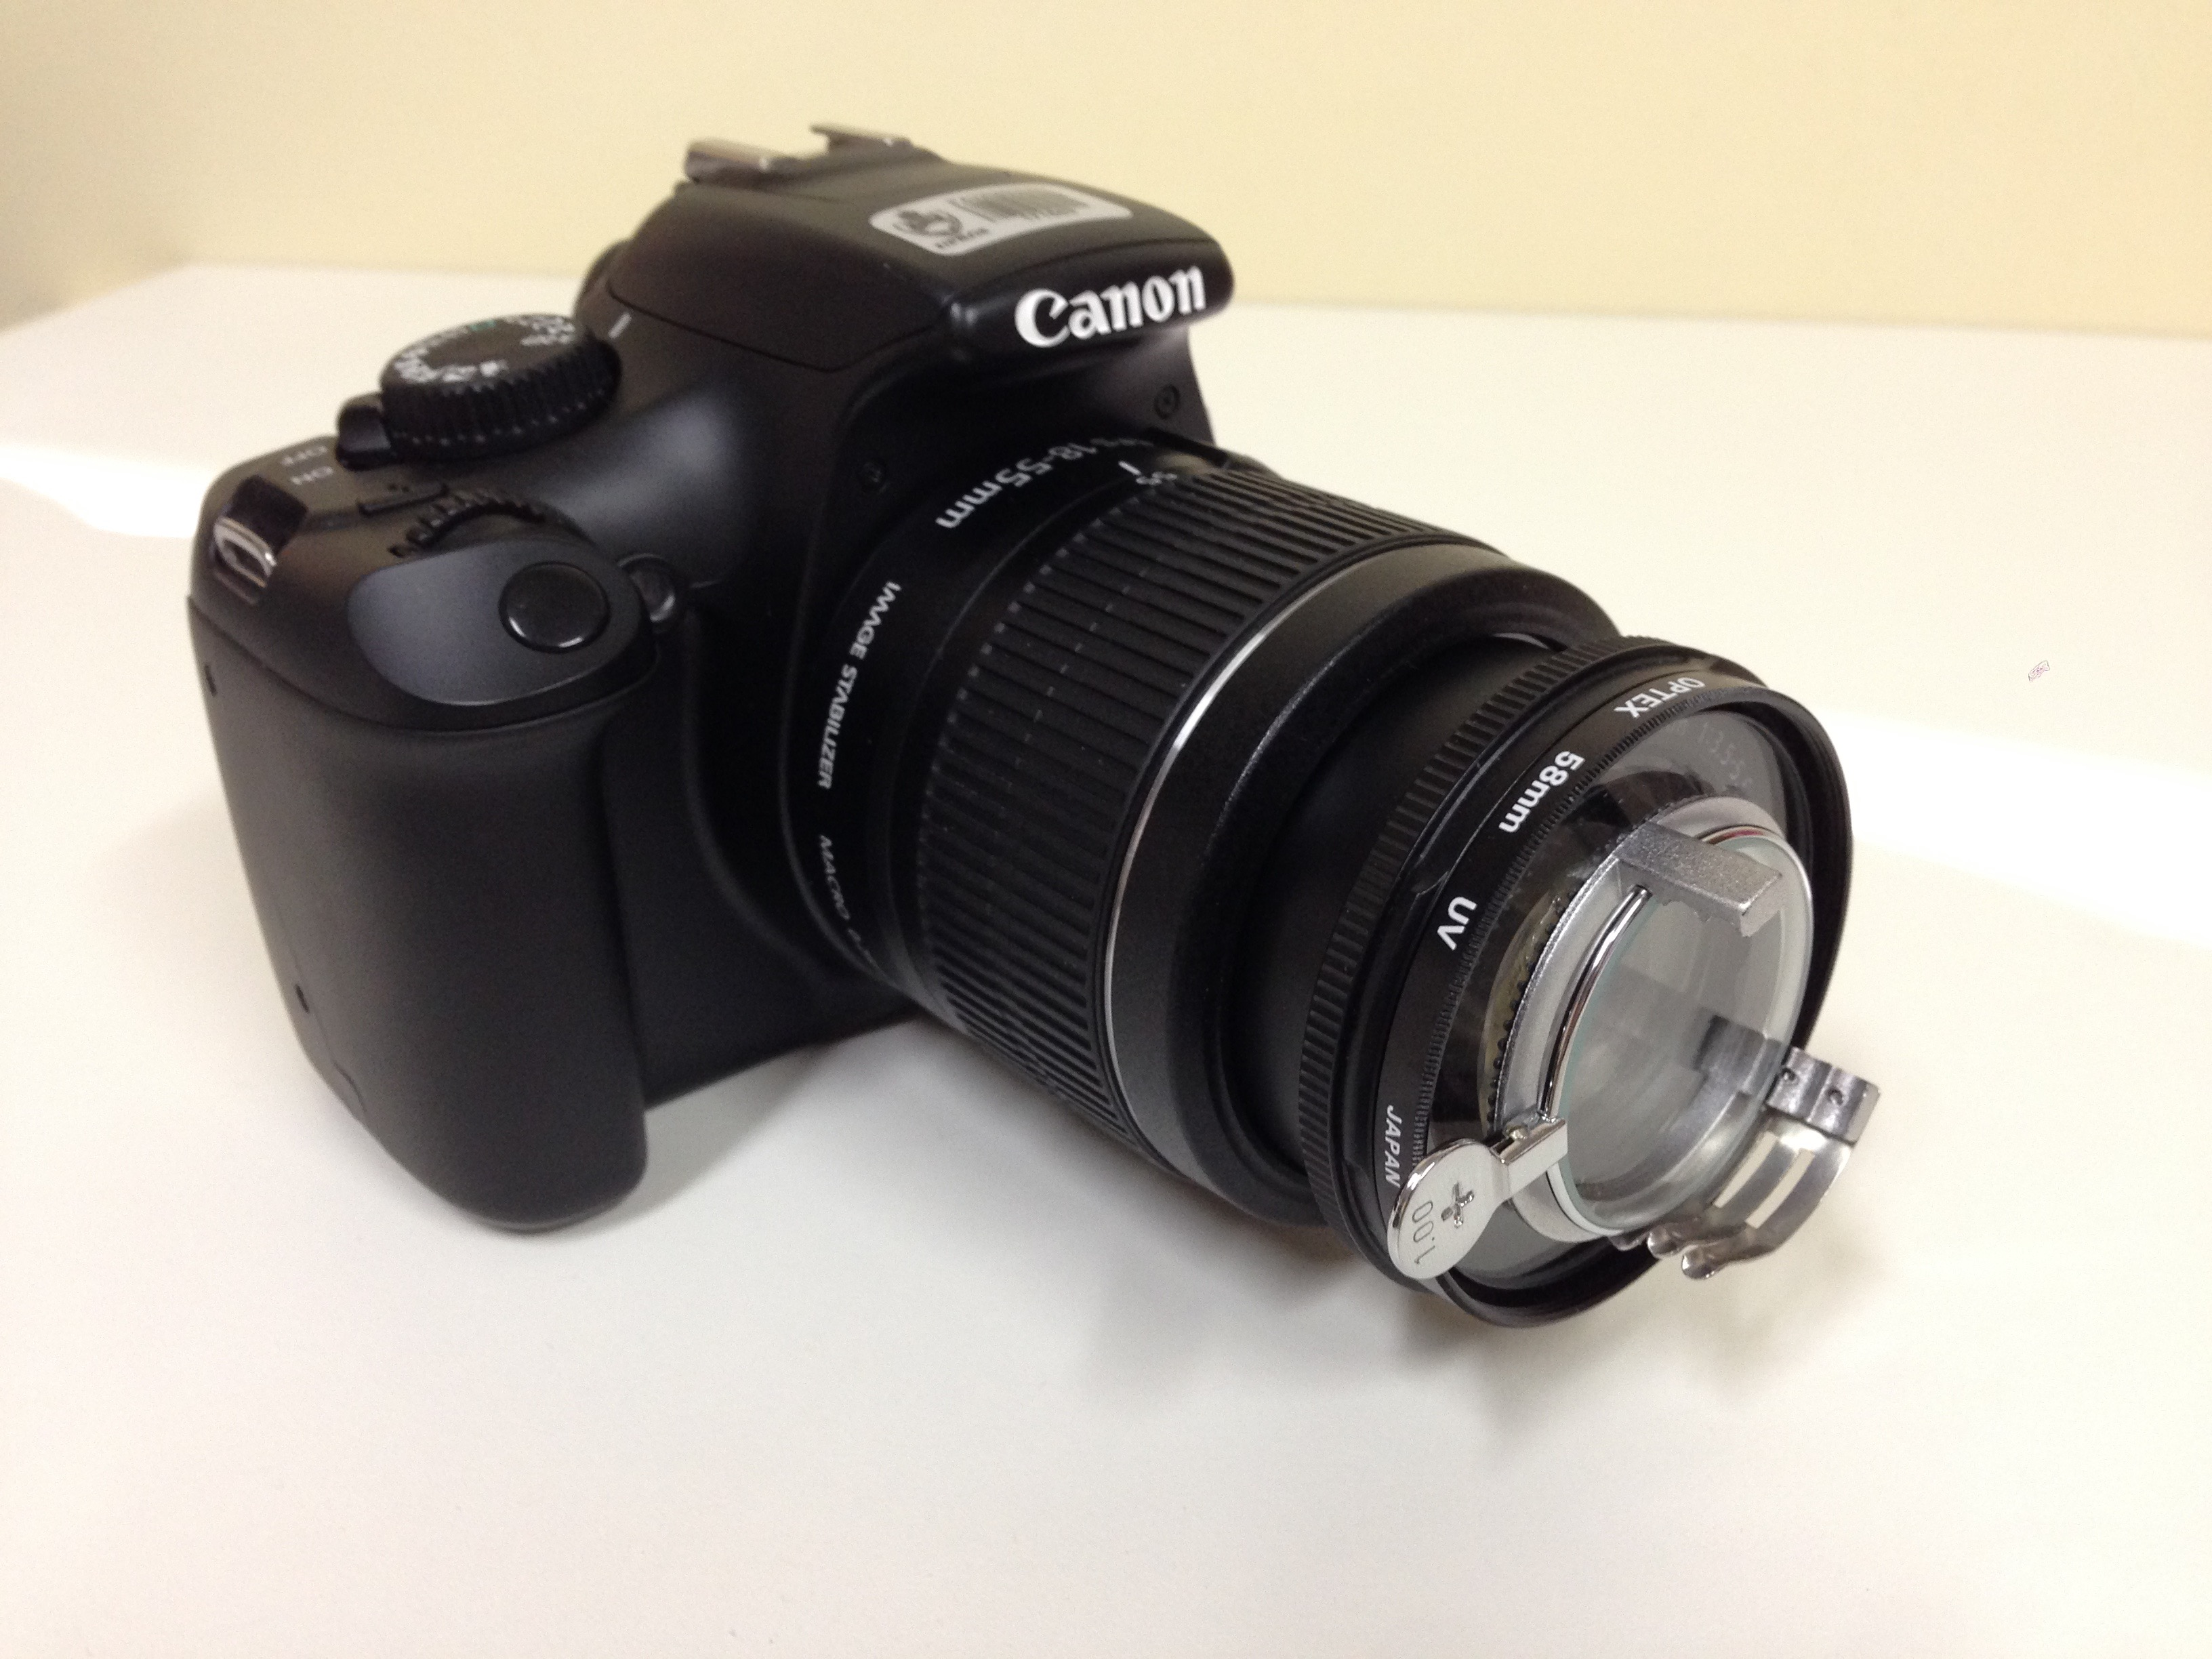
\includegraphics[width=.58\linewidth]{../../__Images/04/camera.jpg}
  ~
  
\includegraphics[width=.36\linewidth]{../../__Images/04/eyemodel.png}
  \hfill \mbox{}
\caption{Optical systems used in the setup: (right) Canon EOS Rebel T3 with apparatus to add up to three extra lenses. Focal lens set to 18mm. (left) Simplified eye model with effective focal length of 13.5mm. {\bf N} is the nodal point.}
	\label{fig:camera}
\end{figure*}

%\begin{figure}[h]
%	\centering
%	
%	\subfigure{
%		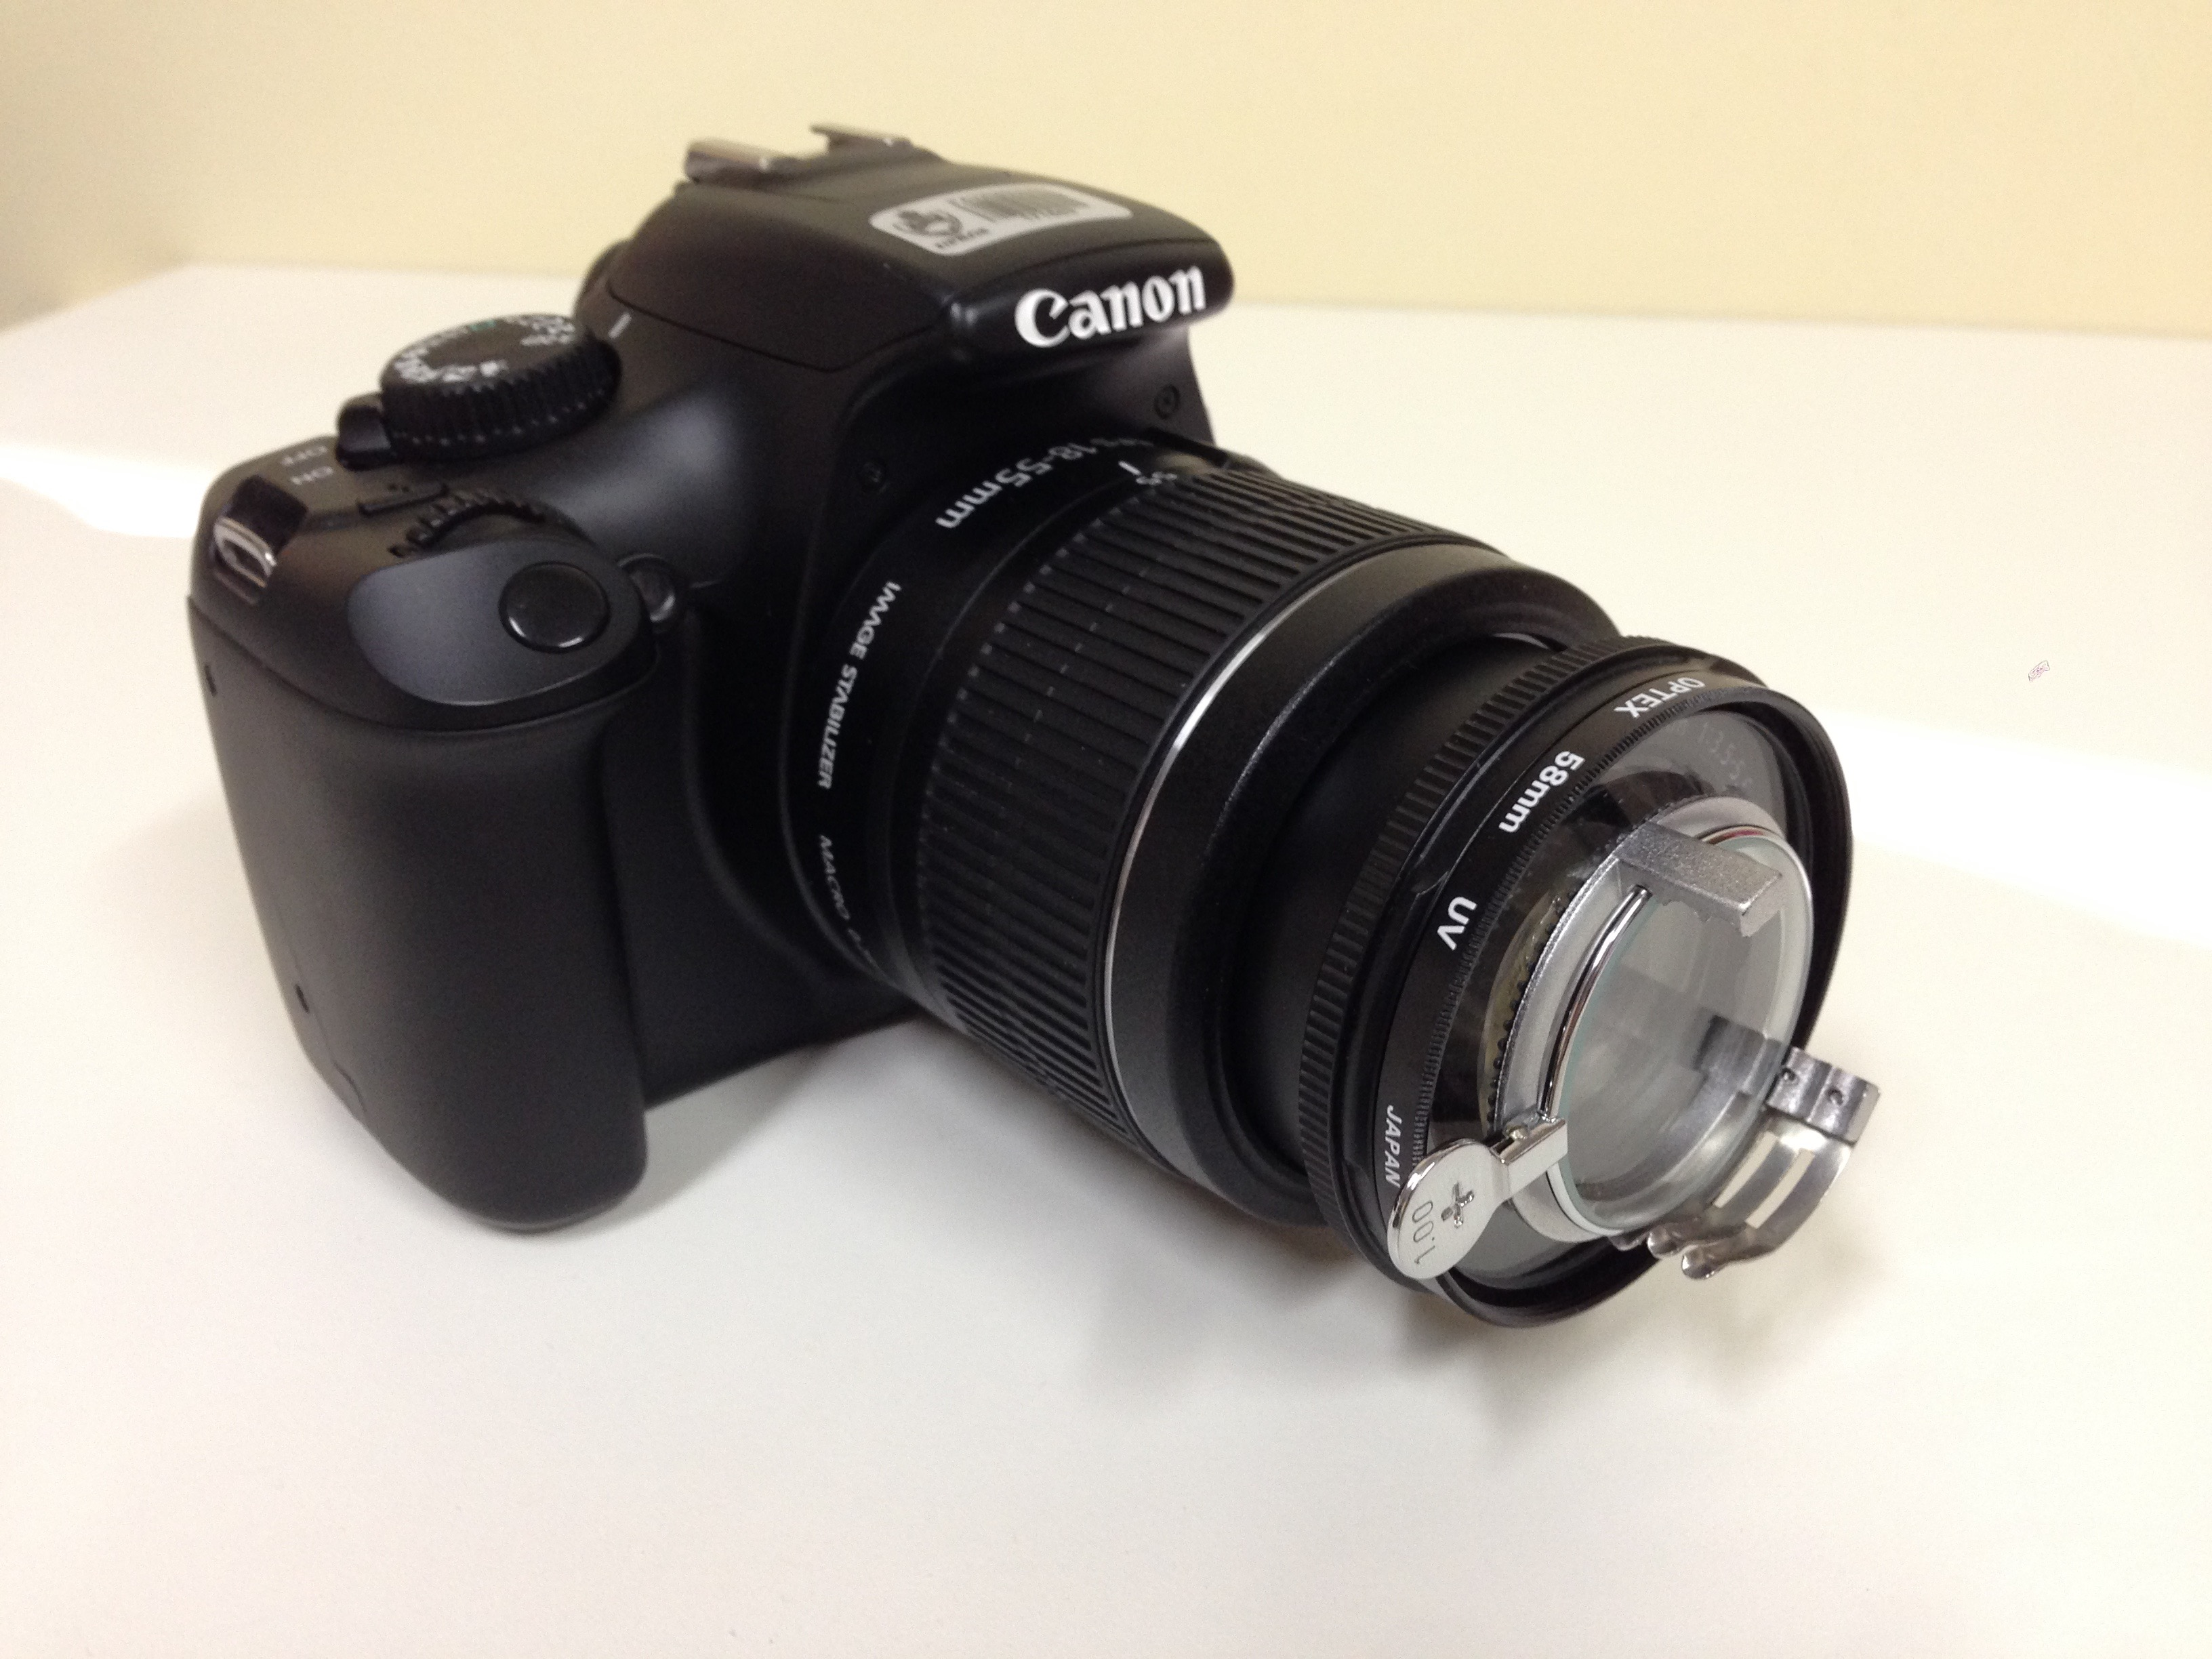
\includegraphics[width=1.00\linewidth]{../../__Images/04/camera.jpg}
%	}
%	~
%	\subfigure{
%		
\includegraphics[width=1.00\linewidth]{../../__Images/04/eyemodel.png}
%	}
%	
%	\caption{Optical systems used in the setup: (top) Canon EOS Rebel T3 with apparatus to add up to three extra lenses. Focal lens set to 18mm. (bottom) Simplified eye model with effective focal length of 13.5mm. {\bf N} is the nodal point.}
%	\label{fig:camera}
%\end{figure}

%-------------------------------------------------------------------------

\subsection{Vertex Distance and Ray Transfer Matrix}

The optical power of a lens prescribed for correcting low-order aberrations varies according to the distance from the lens to the cornea, also known as \emph{vertex distance}. To compensate for the spacing between camera's main lens and the additional ones, we use a \emph{ray transfer matrix} (RTM) formulation \cite{Glytsis2014}. The RTM representing two thin lenses separated by a distance $d$ can be obtained multiplying three matrices: a thin lens matrix (that approximates the DSLR's optical system by a single thin lens), a distance $d$ propagation matrix, and a thin lens matrix representing our additional lenses:
 
\begin{equation}
	\centering
	\label{eq:RTM_tl}
	\begin{array} {lcl} \begin{bmatrix} A_{TL} & B_{TL}\\ C_{TL} & D_{TL} \end{bmatrix} 
	& = & \begin{bmatrix} 1 & 0\\ -\frac{1}{f_{camera}} & 1 \end{bmatrix}
	\begin{bmatrix} 1 & d\\ 0 & 1 \end{bmatrix}
	\begin{bmatrix} 1 & 0\\ -\frac{1}{f_{lens}} & 1 \end{bmatrix} \\ \\ 
	& = & \begin{bmatrix}
	1 - \dfrac{d}{f_{camera}} & d\\
	\left (  \dfrac{\dfrac{d}{f_{lens}}-1}{f_{camera}} - \dfrac{1}{f_{lens}}\right ) & 1 - \dfrac{d}{f_{lens}}
	\end{bmatrix}. 
	\end{array}
\end{equation}

Here $f_{camera}$ is the DLSR camera focal length (\ie, 18mm in our case), and $f_{lens}$ is the focal length of the (combined set of) additional lens(es).
The image captured by the resulting optical system is formed at a distance $x$ behind the DSLR camera's optical system. Assuming we want to capture the image of an infinitely far away object (\eg, at distance $s = 10^{20}$mm from the camera), the overall RTM can computed as:

\begin{equation}
	\centering
	\label{eq:RTM_final}
	\begin{bmatrix} A & B\\ C & D \end{bmatrix}
	=
	\begin{bmatrix} 1 & x\\ 0 & 1 \end{bmatrix}
	\begin{bmatrix} A_{TL} & B_{TL}\\ C_{TL} & D_{TL} \end{bmatrix}
	\begin{bmatrix} 1 & s\\ 0 & 1 \end{bmatrix}.
\end{equation}

Since a set of parallel rays (of an infinitely far away object) are focused by a lens to its focal point, one concludes that $x$ should indeed be the focal length $f_{cam+lens}$ of the compounded optical system comprised by the camera's main lens plus the additional one. By letting $B = 0$, one can solve for $x$, obtaining:

\begin{equation}
	\centering
	\begin{array}{lcl}
	x & = & f_{cam+lens} \\
	  & = & \dfrac{(d  + s) \times (f_{camera} \times f_{lens}) - (d \times f_{lens} \times s) }{(d - f_{lens}) \times f_{camera} + (f_{camera} + f_{lens} - d )\times s}. 
	\end{array}
	\label{RTMx}
\end{equation}

Since 1 diopter = 1/meter, and $f_{cam+lens}$ is expressed in mm, the dioptric power of the resulting compounding optical system is given by:

\begin{equation}
	\centering
	\label{eq:newD}
	diopt_{cam+lens}= \frac{1}{f_{cam+lens} \times 10^{-3}} =  \frac{10^3}{f_{cam+lens}} D.
\end{equation}

Table~\ref{table:newDioptricPower} shows the actual increase in dioptric power that result from placing additional lenses with different powers in front of the camera's main lens, considering a vertex distance of $10mm$. Thus, for instance, when placing a +1.0D lens in front of the camera's main lens, we are in fact inducing myopia of 1.0101D. Therefore, in order to obtain an image comparable to the one captured by the camera, our simulation should compute a wavefront aberration corresponding to 1.0101D of myopia.    

\begin{table}[!h]
\centering
\caption{Actual increase in dioptric power obtained by placing additional lenses with various powers in front of the camera's main lens considering a vertex distance of 10mm.}
\label{table:newDioptricPower}
\begin{tabular}{cc}
\hline
{\bf Additional Lens' dioptric power} & {\bf Actual dioptric power} \\ \hline
0.0000 D                              & 0.0000 D                              \\
1.0000 D                              & 1.0101 D                              \\
2.0000 D                              & 2.0408 D                              \\
3.0000 D                              & 3.0928 D                              \\
4.0000 D                              & 4.1667 D                              \\ \hline
\end{tabular}
\end{table}

%-------------------------------------------------------------------------
\section{Results}


\begin{figure*}[!th]
	\centering

	\begin{tabular}{@{}r@{ } c@{ } c@{ } c@{ } c@{ } c }
	&
	\small{-0.00 D} &
	\small{-1.00 D} &
	\small{-2.00 D} &
	\small{-3.00 D} &
	\small{-4.00 D} & \\

	\begin{sideways} \parbox[b]{20mm} {Camera} \end{sideways} &
	
\includegraphics[width=0.185\textwidth]{../../__Images/05/WB_N(20-200)_-0D_to_-4D/wb_N_20-200_Camera-0,00D(lens).png} &
	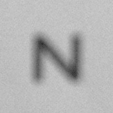
\includegraphics[width=0.185\textwidth]{../../__Images/05/WB_N(20-200)_-0D_to_-4D/wb_N_20-200_Camera-1,00D(lens).png} &
	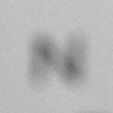
\includegraphics[width=0.185\textwidth]{../../__Images/05/WB_N(20-200)_-0D_to_-4D/wb_N_20-200_Camera-2,00D(lens).png} &
	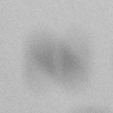
\includegraphics[width=0.185\textwidth]{../../__Images/05/WB_N(20-200)_-0D_to_-4D/wb_N_20-200_Camera-3,00D(lens).png} &
	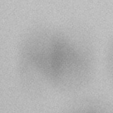
\includegraphics[width=0.185\textwidth]{../../__Images/05/WB_N(20-200)_-0D_to_-4D/wb_N_20-200_Camera-4,00D(lens).png} \\

	\begin{sideways} \parbox[b]{20mm} {Simulation} \end{sideways} &
	
\includegraphics[width=0.185\textwidth]{../../__Images/05/WB_N(20-200)_-0D_to_-4D/wb_N_20-200_Camera-0,00D(simulated).png} &
	
\includegraphics[width=0.185\textwidth]{../../__Images/05/WB_N(20-200)_-0D_to_-4D/wb_N_20-200_Camera-1,00D(simulated).png} &
	
\includegraphics[width=0.185\textwidth]{../../__Images/05/WB_N(20-200)_-0D_to_-4D/wb_N_20-200_Camera-2,00D(simulated).png} &
	
\includegraphics[width=0.185\textwidth]{../../__Images/05/WB_N(20-200)_-0D_to_-4D/wb_N_20-200_Camera-3,00D(simulated).png} &
	
\includegraphics[width=0.185\textwidth]{../../__Images/05/WB_N(20-200)_-0D_to_-4D/wb_N_20-200_Camera-4,00D(simulated).png} \\

	\begin{sideways} \parbox[b]{20mm} {Local~SSIM} \end{sideways} &
	
\includegraphics[width=0.185\textwidth]{../../__Images/05/WB_N(20-200)_-0D_to_-4D/wb_N_20-200_Camera-0,00D(comparison).png} &
	
\includegraphics[width=0.185\textwidth]{../../__Images/05/WB_N(20-200)_-0D_to_-4D/wb_N_20-200_Camera-1,00D(comparison).png} &
	
\includegraphics[width=0.185\textwidth]{../../__Images/05/WB_N(20-200)_-0D_to_-4D/wb_N_20-200_Camera-2,00D(comparison).png} &
	
\includegraphics[width=0.185\textwidth]{../../__Images/05/WB_N(20-200)_-0D_to_-4D/wb_N_20-200_Camera-3,00D(comparison).png} &
	
\includegraphics[width=0.185\textwidth]{../../__Images/05/WB_N(20-200)_-0D_to_-4D/wb_N_20-200_Camera-4,00D(comparison).png} \\
	
	\begin{sideways} \parbox[b]{20mm} {Absolute Difference} \end{sideways} &
	
\includegraphics[width=0.185\textwidth]{../../__Images/05/WB_N(20-200)_-0D_to_-4D/wb_N_20-200_Camera-0,00D(diff).png} &
	
\includegraphics[width=0.185\textwidth]{../../__Images/05/WB_N(20-200)_-0D_to_-4D/wb_N_20-200_Camera-1,00D(diff).png} &
	
\includegraphics[width=0.185\textwidth]{../../__Images/05/WB_N(20-200)_-0D_to_-4D/wb_N_20-200_Camera-2,00D(diff).png} &
	
\includegraphics[width=0.185\textwidth]{../../__Images/05/WB_N(20-200)_-0D_to_-4D/wb_N_20-200_Camera-3,00D(diff).png} &
	
\includegraphics[width=0.185\textwidth]{../../__Images/05/WB_N(20-200)_-0D_to_-4D/wb_N_20-200_Camera-4,00D(diff).png} \\
 
	\end{tabular}
	
	\caption{Comparisons of our simulated results against ground truth obtained with a hyperopic camera. These large images correspond to a Snellen ratio of 20/200. (top row) Images captured using the DSLR camera with extra lenses varying from 0.0 to -4.0 diopters. (second row) Our simulated results. (third row) SSIM metric results. (fourth row) AD metric.}
	\label{fig:comparison_hyperopic_wb}
\end{figure*}

\begin{figure*}[!th]
	\centering
	
	\begin{tabular}{@{}r@{ } c@{ } c@{ } c@{ } c@{ } c }
	&
	\small{+0.00 D} &
	\small{+1.00 D} &
	\small{+2.00 D} &
	\small{+3.00 D} &
	\small{+4.00 D} & \\

	\begin{sideways} \parbox[b]{20mm} {Camera} \end{sideways} &
	
\includegraphics[width=0.185\textwidth]{../../__Images/05/BW_N(20-200)_+0D_to_+4D/bw_N_20-200_Camera+0,00D(lens).png} &
	
\includegraphics[width=0.185\textwidth]{../../__Images/05/BW_N(20-200)_+0D_to_+4D/bw_N_20-200_Camera+1,00D(lens).png} &
	
\includegraphics[width=0.185\textwidth]{../../__Images/05/BW_N(20-200)_+0D_to_+4D/bw_N_20-200_Camera+2,00D(lens).png} &
	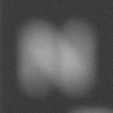
\includegraphics[width=0.185\textwidth]{../../__Images/05/BW_N(20-200)_+0D_to_+4D/bw_N_20-200_Camera+3,00D(lens).png} &
	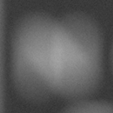
\includegraphics[width=0.185\textwidth]{../../__Images/05/BW_N(20-200)_+0D_to_+4D/bw_N_20-200_Camera+4,00D(lens).png} \\

	\begin{sideways} \parbox[b]{20mm} {Simulation} \end{sideways} &
	
\includegraphics[width=0.185\textwidth]{../../__Images/05/BW_N(20-200)_+0D_to_+4D/bw_N_20-200_Camera+0,00D(simulated).png} &
	
\includegraphics[width=0.185\textwidth]{../../__Images/05/BW_N(20-200)_+0D_to_+4D/bw_N_20-200_Camera+1,00D(simulated).png} &
	
\includegraphics[width=0.185\textwidth]{../../__Images/05/BW_N(20-200)_+0D_to_+4D/bw_N_20-200_Camera+2,00D(simulated).png} &
	
\includegraphics[width=0.185\textwidth]{../../__Images/05/BW_N(20-200)_+0D_to_+4D/bw_N_20-200_Camera+3,00D(simulated).png} &
	
\includegraphics[width=0.185\textwidth]{../../__Images/05/BW_N(20-200)_+0D_to_+4D/bw_N_20-200_Camera+4,00D(simulated).png} \\

	\begin{sideways} \parbox[b]{20mm} {Local~SSIM} \end{sideways} &
	
\includegraphics[width=0.185\textwidth]{../../__Images/05/BW_N(20-200)_+0D_to_+4D/bw_N_20-200_Camera+0,00D(comparison).png} &
	
\includegraphics[width=0.185\textwidth]{../../__Images/05/BW_N(20-200)_+0D_to_+4D/bw_N_20-200_Camera+1,00D(comparison).png} &
	
\includegraphics[width=0.185\textwidth]{../../__Images/05/BW_N(20-200)_+0D_to_+4D/bw_N_20-200_Camera+2,00D(comparison).png} &
	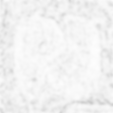
\includegraphics[width=0.185\textwidth]{../../__Images/05/BW_N(20-200)_+0D_to_+4D/bw_N_20-200_Camera+3,00D(comparison).png} &
	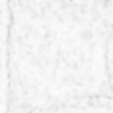
\includegraphics[width=0.185\textwidth]{../../__Images/05/BW_N(20-200)_+0D_to_+4D/bw_N_20-200_Camera+4,00D(comparison).png} \\
	
	\begin{sideways} \parbox[b]{20mm} {Absolute Difference} \end{sideways} &
	
\includegraphics[width=0.185\textwidth]{../../__Images/05/BW_N(20-200)_+0D_to_+4D/bw_N_20-200_Camera+0,00D(diff).png} &
	
\includegraphics[width=0.185\textwidth]{../../__Images/05/BW_N(20-200)_+0D_to_+4D/bw_N_20-200_Camera+1,00D(diff).png} &
	
\includegraphics[width=0.185\textwidth]{../../__Images/05/BW_N(20-200)_+0D_to_+4D/bw_N_20-200_Camera+2,00D(diff).png} &
	
\includegraphics[width=0.185\textwidth]{../../__Images/05/BW_N(20-200)_+0D_to_+4D/bw_N_20-200_Camera+3,00D(diff).png} &
	
\includegraphics[width=0.185\textwidth]{../../__Images/05/BW_N(20-200)_+0D_to_+4D/bw_N_20-200_Camera+4,00D(diff).png} \\
 
	\end{tabular}
	
	\caption{Comparisons of our simulated results against ground truth obtained with a myopic camera. These large images correspond to a Snellen ratio of 20/200. (top row) Images captured using the DSLR camera with extra lenses varying from 0.0 to 4.0 diopters. (second row) Our simulated results. (third row) SSIM metric results. (fourth row) AD metric.}
	\label{fig:comparison_myopic_bw}
\end{figure*}

This section compares our simulated results with an optical ground truth, obtained by capturing images of the LogMAR charts with a DSLR camera set up for $f/5.0$ (third row of Table~\ref{table:pupildiameter}), although other values could have been used. Whenever we reference to the dioptric power of additional lenses, our simulations account for the values described in Table~\ref{table:newDioptricPower}. To objectively evaluate the quality of the simulated results, we use three objective metrics: the Structural Similarity Image Metric (SSIM)~\cite{Wang2004}, the Peak Signal-to-Noise Ratio (PSNR), and the Absolute Difference (AD) of the pixelwise differences between the captured and simulated images. The SSIM metric measures image degradation perceived as change in structural information. It is calculated for each pixel of a given image with respect to some reference image, based on its relationship to other pixels in an 11-by-11 neighborhood. PSNR is a popular metric in image processing for assessing the quality of image reconstruction and compression. It is often expressed using a decibel scale, and computed as  

\begin{equation}
	\centering
	\label{eq:PSNR}
	PSNR = 10\log_{10}\left (\frac{peakval^2}{MSE}\right ),
\end{equation}
where
\begin{equation}
	\centering
	\label{eq:MSE}
	MSE = \frac{1}{mn}\sum^{m-1}_{i=0}\sum^{n-1}_{j=0}(I_{ref}(i,j) - I(i,j))^2,
\end{equation}
and $I$ is an image being compared to a reference image $I_{ref}$, both with the same dimensions $m \times n$. 
$peakval$ is the maximum possible value for a pixel. For instance, for a grayscale image using 8-bits per pixel, $peakval=255$. 


Fig.~\ref{fig:comparison_hyperopic_wb} and \ref{fig:comparison_myopic_bw} compare images of a letter from the LogMAR charts with white and black background, respectively, captured by the DSLR camera (top row) against the results of our simulations (second row). The images in the top rows were captured by the camera with additional lenses, ranging from 0 to -4 diopters (Fig.~\ref{fig:comparison_hyperopic_wb}) or from 0 to +4 diopters (Fig.~\ref{fig:comparison_myopic_bw}), in steps of 1 diopter. The second rows show the images produced using our simulation and considering the adjustments in dioptric power required to account for the 10mm spacing between the camera's main lens and the additional one (Table~\ref{table:newDioptricPower}). Our simulations were applied to the image captured by the camera without any extra lens (\ie, camera +0.00 D). The third and fourth rows of these figures show visual representations of the SSIM an AD metrics, respectively.

Tables~\ref{table:hyperopic} and \ref{table:myopic} show the numerical results of the SSIM and PSNR metrics for the results presented in Fig.~\ref{fig:comparison_hyperopic_wb} and \ref{fig:comparison_myopic_bw}, respectively. Each row represents the value of a specific metric (\ie, SSIM or PSNR) when comparing an image captured by the DSLR camera with the one obtained using our simulation. The values of the SSIM metric range from -1.0 (poor similarity) to 1.0 (high similarity). In these tables, one can see that all values are very close to 1.0, indicating that our simulations indeed produces results that are structurally very  similar the ground truth. The PSNR values also indicate that our simulations also produce results very similar to the ground truth. Note that PSNR values of 34.0 and above indicate that two images are essentially indistinguishable from each other.  

~


\begin{table}[!hb]
	\centering
	\caption{SSIM and PSNR table of the hyperopic perception}%(Fig.~\ref{fig:comparison_hyperopic_wb})
		\label{table:hyperopic}
	\scalebox{0.85}{
	\begin{tabular}{cccccc}
	{ }                          & \textbf{0.00 D} & \textbf{-1.00 D} & \textbf{-2.00 D} & \textbf{-3.00 D} & \textbf{-4.00 D} \\ \hline
	\multicolumn{1}{c|}{\textbf{SSIM}} & 0.9869  		& 0.9192  		& 0.9149  		& 0.9119  		& 0.9130  		\\
	\multicolumn{1}{c|}{\textbf{PSNR}} & 34.7778 		& 34.3781 		& 32.8601 		& 32.6680 		& 29.5003
	\end{tabular}
	}
\end{table}

\begin{table}[!hb]
	\centering
	\caption{SSIM and PSNR table of the myopic perception}%(Fig.~\ref{fig:comparison_myopic_bw})
		\label{table:myopic}
		\scalebox{0.85}{
	\begin{tabular}{cccccc}
	{}                          & \textbf{0.00 D} & \textbf{1.00 D} & \textbf{2.00 D} & \textbf{3.00 D} & \textbf{4.00 D} \\ \hline
	\multicolumn{1}{c|}{\textbf{SSIM}} & 0.9869  		& 0.9378  		& 0.9324  		& 0.9296  		& 0.9322  		\\
	\multicolumn{1}{c|}{\textbf{PSNR}} & 34.7779 		& 38.8748 		& 38.7219 		& 35.6993 		& 39.3720
	\end{tabular}
	}
\end{table}



		%\review{\lipsum[7-8]}




\begin{figure*}[!bht]
	\centering

	\begin{tabular}{@{}r@{ } c@{ } c@{ } c@{ } c@{ } c }
%	&
%	\small{N} &
%	\small{C} &
%	\small{K} &
%	\small{Z} &
%	\small{O} & \\

	\begin{sideways} \parbox[b]{20mm} {Camera} \end{sideways} &
	
\includegraphics[width=0.185\textwidth]{../../__Images/05/BW_20-200_+2@90/bw_N_20-200_Camera+2,00D@90(lens).png} &
	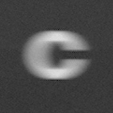
\includegraphics[width=0.185\textwidth]{../../__Images/05/BW_20-200_+2@90/bw_C_20-200_Camera+2,00D@90(lens).png} &
	\includegraphics[width=0.185\textwidth]{../../__Images/05/BW_20-200_+2@90/bw_K_20-200_Camera+2,00D@90(lens).png} &
	\includegraphics[width=0.185\textwidth]{../../__Images/05/BW_20-200_+2@90/bw_Z_20-200_Camera+2,00D@90(lens).png} &
	\includegraphics[width=0.185\textwidth]{../../__Images/05/BW_20-200_+2@90/bw_O_20-200_Camera+2,00D@90(lens).png} \\

	\begin{sideways} \parbox[b]{20mm} {Simulation} \end{sideways} &
	\includegraphics[width=0.185\textwidth]{../../__Images/05/BW_20-200_+2@90/bw_N_20-200_Camera+2,00D@90(simulated).png} &
	\includegraphics[width=0.185\textwidth]{../../__Images/05/BW_20-200_+2@90/bw_C_20-200_Camera+2,00D@90(simulated).png} &
	\includegraphics[width=0.185\textwidth]{../../__Images/05/BW_20-200_+2@90/bw_K_20-200_Camera+2,00D@90(simulated).png} &
	\includegraphics[width=0.185\textwidth]{../../__Images/05/BW_20-200_+2@90/bw_Z_20-200_Camera+2,00D@90(simulated).png} &
	\includegraphics[width=0.185\textwidth]{../../__Images/05/BW_20-200_+2@90/bw_O_20-200_Camera+2,00D@90(simulated).png} \\

	\begin{sideways} \parbox[b]{20mm} {Local~SSIM} \end{sideways} &
	\includegraphics[width=0.185\textwidth]{../../__Images/05/BW_20-200_+2@90/bw_N_20-200_Camera+2,00D@90(comparison).png} &
	\includegraphics[width=0.185\textwidth]{../../__Images/05/BW_20-200_+2@90/bw_C_20-200_Camera+2,00D@90(comparison).png} &
	\includegraphics[width=0.185\textwidth]{../../__Images/05/BW_20-200_+2@90/bw_K_20-200_Camera+2,00D@90(comparison).png} &
	\includegraphics[width=0.185\textwidth]{../../__Images/05/BW_20-200_+2@90/bw_Z_20-200_Camera+2,00D@90(comparison).png} &
	\includegraphics[width=0.185\textwidth]{../../__Images/05/BW_20-200_+2@90/bw_O_20-200_Camera+2,00D@90(comparison).png} \\
	
	\begin{sideways} \parbox[b]{20mm} {Absolute Difference} \end{sideways} &
	\includegraphics[width=0.185\textwidth]{../../__Images/05/BW_20-200_+2@90/bw_N_20-200_Camera+2,00D@90(diff).png} &
	\includegraphics[width=0.185\textwidth]{../../__Images/05/BW_20-200_+2@90/bw_C_20-200_Camera+2,00D@90(diff).png} &
	\includegraphics[width=0.185\textwidth]{../../__Images/05/BW_20-200_+2@90/bw_K_20-200_Camera+2,00D@90(diff).png} &
	\includegraphics[width=0.185\textwidth]{../../__Images/05/BW_20-200_+2@90/bw_Z_20-200_Camera+2,00D@90(diff).png} &
	\includegraphics[width=0.185\textwidth]{../../__Images/05/BW_20-200_+2@90/bw_O_20-200_Camera+2,00D@90(diff).png} \\

	\end{tabular}
	
	\caption{Comparisons of our simulated results against ground truth obtained with a astigmatic camera. These large images correspond to a Snellen ratio of 20/200. (top row) Images captured using the DSLR camera with an extra cylindrical lens with 2 diopters at the vertical meridian. (second row) Our simulated results. (third row) SSIM metric results. (fourth row) AD metric.}
	\label{fig:astig}
\end{figure*}



\begin{table}[!hb]
	\centering
	\caption{SSIM and PSNR table of the astigmatic perception}%(Fig.~\ref{fig:astig})
	\label{table:metrics_astig}
%	\caption{SSIM and PSNR table BW astigmatism +2 @90}
	\scalebox{0.85}{
		\begin{tabular}{cccccc}
		{\bf }                          & \textbf{N} & \textbf{C} & \textbf{K} & \textbf{Z} & \textbf{O} \\ \hline
		\multicolumn{1}{c|}{\textbf{SSIM}} & 0.9307  & 0.9271  & 0.9277  & 0.9193  & 0.9303  		\\
		\multicolumn{1}{c|}{\textbf{PSNR}} & 37.2835 & 35.4130 & 36.3713 & 32.7150 & 36.2564
	\end{tabular}
	}
\end{table}
% !TEX root = ./../../../_Thesis.tex

\begin{figure*}[h]
	\centering

	\begin{tabular}{@{}r@{ } c@{ } c@{ } c@{ } c@{ } c }
	&
	\small{Input Letter} &
	\small{Aberrated Wavefront} &
	\small{Spatial PSF} &
	\small{Simulation} & \\ \\

	\begin{sideways} \parbox[b]{25mm} {} \end{sideways} &
	\includegraphics[width= 0.22\textwidth]{__Images/05/synthetic_sims/C_20-200@4x.png} &
	\includegraphics[height=0.22\textwidth]{__Images/05/synthetic_sims/Wavefront_0,5D,-2@45.png} &
	\includegraphics[width= 0.22\textwidth]{__Images/05/synthetic_sims/PSF_0,5D,-2@45.png} &
	\includegraphics[width= 0.22\textwidth]{__Images/05/synthetic_sims/C_20-200_f50_simulated(0,5D,-2@45).png} 			\\ \\

	\begin{sideways} \parbox[b]{25mm} {} \end{sideways} &
	\includegraphics[width= 0.22\textwidth]{__Images/05/synthetic_sims/O_20-200@4x.png} &
	\includegraphics[height=0.22\textwidth]{__Images/05/synthetic_sims/Wavefront_0D,-4,7@135.png} &
	\includegraphics[width= 0.22\textwidth]{__Images/05/synthetic_sims/PSF_0D,-4,7@135.png} &
	\includegraphics[width= 0.22\textwidth]{__Images/05/synthetic_sims/O_20-200_f50_simulated(0D,-4,7@135).png}			\\ \\

	\begin{sideways} \parbox[b]{25mm} {} \end{sideways} &
	\includegraphics[width= 0.22\textwidth]{__Images/05/synthetic_sims/R_20-200@4x.png} &
	\includegraphics[height=0.22\textwidth]{__Images/05/synthetic_sims/Wavefront_6D,0@0.png} &
	\includegraphics[width= 0.22\textwidth]{__Images/05/synthetic_sims/PSF_6D,0@0.png} &
	\includegraphics[width= 0.22\textwidth]{__Images/05/synthetic_sims/R_20-200_f50_simulated(6D,0@0).png}				\\ \\
	
	\begin{sideways} \parbox[b]{25mm} {} \end{sideways} &
	\includegraphics[width= 0.22\textwidth]{__Images/05/synthetic_sims/S_20-200@4x.png} &
	\includegraphics[height=0.22\textwidth]{__Images/05/synthetic_sims/Wavefront_highorder.png} &
	\includegraphics[width= 0.22\textwidth]{__Images/05/synthetic_sims/PSF_highorder.png} &
	\includegraphics[width= 0.22\textwidth]{__Images/05/synthetic_sims/S_20-200_f50_simulated(high-order).png}			\\

	\end{tabular}
	
	\caption[Simulations with arbitrary wavefronts]{Simulations with arbitrary wavefronts. The input letter images correspond to a Snellen ratio of 20/200. (second column) Normalized aberrated wavefront. (third column) The spatial PSF. (fourth column) Our simulation results given the images shown in column \emph{Input Letter}. The top row shows how a combination of low-order aberrations (+0.5 Sph. -2.0 Cyl. at 45$^{\circ}$) affects the perception of a Sloan letter. The second and third rows simulate, respectively, higher values of pure astigmatism and spherical aberration (-4.7 Cyl. at 135$^{\circ}$ and +6 Sph.) than one can capture with the lenses available in our trial lens set. The bottom row shows the results of a simulation involving only higher-order aberrations ($Z^{-3}_{3}=0.2$, $Z^{-1}_{3}=0.2$, $Z^{3}_{3}=0.1$, $Z^{2}_{4}=0.2$, $Z^{-5}_{5}=0.4$, $Z^{1}_{5}=0.3$).}
	\label{fig:synthetic_sims}
\end{figure*}

\clearpage


Besides simulating the effects of defocus (\ie, myopia and hyperopia), we have also compared the results of our simulation for astigmatic vision.
%We've also explored simulations of more effects rather than defocus. 
This is illustrated in Fig.~\ref{fig:astig}.
% shows the simulation of an astigmatic perception. 
The Sloan letters in Fig.~~\ref{fig:astig} were captured by the DSLR camera with an additional cylindrical lens with 2.0 diopters, rotated in order to simulate astigmatism in the horizontal meridian ($\phi = 90^{\circ}$).
Table~\ref{table:metrics_astig} shows the results of the SSIM and PSNR metrics for these astigmatic results. Again, the SSIM indices are close 1.0 and the PSNR is close to or above 34.00 decibels.
%
Note that for the astigmatic results, part of the differences visible in 
the astigmatic local SSIM index visualizations (Fig.~\ref{fig:astig}(third row)) is due to the difficulty of a precise manual alignment of the astigmatic axes to the ones used in our simulations. Any deviation from the simulated angles affects the results of the quality metric.

%

Our technique can be used to simulate arbitrary wavefront aberrations, given the corresponding aberration function $W_{(x,y)}$ (Equation~\ref{eq:W}). Thus, even though such a validation depends on the existence of an optical ground truth, the method is not limited to what can be modeled using a DSLR camera and additional lenses.
%the ones configured in previous camera's setup. 
Columns \emph{Aberrated Wavefront} and \emph{Spatial PSF} in Figure \ref{fig:synthetic_sims} show the normalized aberrated wavefront and the spatial PSF associated with the simulation results shown in the last column for a given input letter. 
%Figure \ref{fig:synthetic_sims} (top row) 
Its top row shows the results of a simulation involving only higher-order aberrations. 
The bottom row shows how a combination of low-order aberrations (myopia and astigmatism) affects the perception of a Sloan letter. 

%-------------------------------------------------------------------------
\section{Discussion}

This paper described a technique for simulating the visual perception of monochromatic images observed by an optical systems with aberrations. It assumes that all elements of a given target image are at the same known distance from the camera. The technique is based on Fourier optics. We validated the results of our simulations using a DSLR camera with the addition of external lenses to simulate myopia, hyperopia, and astigmatism. Although our solution is able to take into account high-order aberrations, our focus was on not relying on the availability of expensive equipment, such as Shack-Hartmann wavefront sensors. For this, we have focused on simulating low-order aberrations, which can be done directly from the data available on one's eyeglasses prescription.

We have demonstrate the effectiveness of our technique by comparing the results of forty simulations against optical ground truths captured by a camera. For this we used three objective metrics: SSIM, PSNR, and the absolute differences of the images. For all results the SSIM values are between 0.91 and 0.987 (mean = 0.93 and standard deviation = 0.02), indicating that our simulations indeed produce results that are structurally very similar the ground truths. Regarding the PSNR metric, the values vary from 29.50 to 39.37 (mean = 35.50 and standard deviation = 2.14). Such PSNR values, given in decibels, indicate that the simulation outcomes are indistinguishable from the optical ground truth captured by a DSLR camera.

Although the technique itself is not novel, the detailed description presented here consolidates and clarifies information from various sources, providing a valuable resource for the research community.

%------------------------------------------------------------------------
\subsection{Future Work}

Because visual blurring is a depth-dependent phenomenon, we would like to capture image and depth information from the environment and generate real-time simulations of how low-order aberrations affect visual perception. Also, we would like to include information about the absolute threshold in the simulation to improve its result.

For a qualitative validation, it would be desirable to simulate the visual perception of a number of individuals who use eyeglasses. We could then ask these subjects to compare several scenes observed without their eyeglasses with the corresponding simulated views, this time with their eyeglasses on. Such an experiment could indicate how well the simulation approximates their actual vision.

%-------------------------------------------------------------------------

%\subsection{Acknowledgements}

%This work was sponsored by FAPERGS (Funda��o de Amparo � Pesquisa do Rio Grande do Sul) and CAPES-Brazil (Coordena��o de Aperfei�oamento de Pessoal de N�vel Superior).

\bibliographystyle{eg-alpha}
%\bibliographystyle{eg-alpha-doi}

%\bibliography{egbibsample}
\bibliography{Database}
\end{document}

